\chapter{Convolutional Neural Network} \label{chap:cnn}

% Dieses Kapitel geht zunächst detailliert auf den im vorherigen Kapitel eingeführten Begriff Convolutional Neural Network (CNN) ein. Danach wird das Kapitel durch die Betrachtung der ... abgeschlossen.

In diesem Kapitel wird dargestellt, welche Durchbrüche speziell den Anlass zu Convolutional Neural Network (CNN) gegeben haben, wie sich DNN- und CNN-Struktur voneinander unterscheiden und wie CNN-Schichten aus funktionaler Sicht aussehen.

\section{Entwicklungsmeilensteine}

\begin{figure}[!hb]
	\centering
	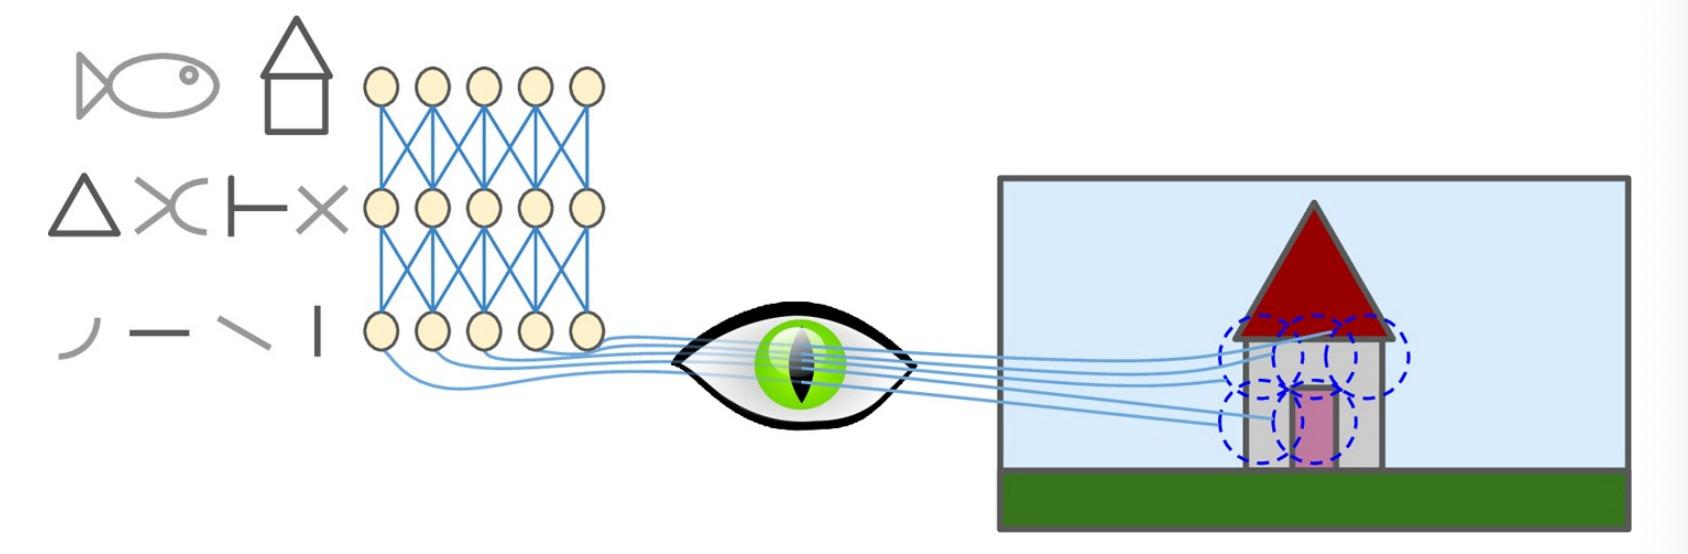
\includegraphics[width=\linewidth]{images/local_receptive_field}
	\caption{Lokales rezeptives Feld im visuellen Cortex \protect\cite{LocalReceptiveField}}
	\label{fig:1959CatExpr}
\end{figure}

\begin{description}
	\item[1959 - 1962]
		
	David H. Hubel und Torsten N. Wiesel untersuchten in \cite{PMID:14403678,PMID:14403679} und danach in \cite{PMID:14449617} durch eine Reihe von Experimenten an Katzen die Struktur vom \emph{visuellen Cortex}, der gemäß \cite{Bergua2017} ''die Region des Gehirns ist, die für die Verarbeitung und Integration der visuellen Information verantwortlich ist'' . Die Autoren entdeckten, dass viele Neuronen im visuellen Cortex ein kleines \emph{lokales rezeptives Feld} haben, d.h. sie reagieren nur auf visuelle Stimuli, die sich in einem begrenzten Bereich des Gesichtsfeldes befinden (siehe \autoref{fig:1959CatExpr}, in der die lokalen rezeptiven Felder von fünf Neuronen durch gestrichelte Kreise dargestellt werden). Die rezeptiven Felder verschiedener Neuronen können sich überlappen und zusammen bilden sie das gesamte Gesichtsfeld. Außerdem fanden Hubel und Wiesel heraus, dass bestimmte Neuronen nur auf bestimmte Arten von visuellen Stimuli reagieren, und dass einige Neuronen größere rezeptive Felder haben sowie auf komplexere Muster reagieren, die Kombinationen einfacherer Muster sind. 
	
	Diese Beobachtungen führten zu der Idee, dass Neuronen eine hierarchische Organisation haben. Insbesondere basieren Neuronen höherer Schichten auf den Ausgaben benachbarter Neuronen in niedrigeren Schichten (Beachte in \autoref{fig:1959CatExpr}, dass jedes Neuron nur mit einigen wenigen Neuronen in der vorherigen Schicht verbunden ist). Diese Idee (im Weiteren als \emph{Hierarchical-Neural-Network-Idee} bezeichnet) schuf das erste wesentliche Fundament für die Entwicklung von CNN.
		
	\item[1980 \& 1988] 
	
	Hubel und Wiesels Studien vom visuellen Cortex gaben Inspiration für das \emph{Neocognitron} von Kunihiko Fukushima, welches das erste Beispiel für eine Netzwerkarchitektur war, die die Hierarchical-Neural-Network-Idee in ihr Design aufnahm. Im Prinzip ist das Neocognitron ein Modell, das 1980 in \cite{Neocognitron1980} für einen Mechanismus der verformungsbeständigen visuellen Mustererkennung vorgeschlagen und später 1988 in \cite{Neocognitron1988} gezeigt wurde, dass es nach Training dazu in der Lage war.
	
	\begin{figure}[!hb]
		\centering
		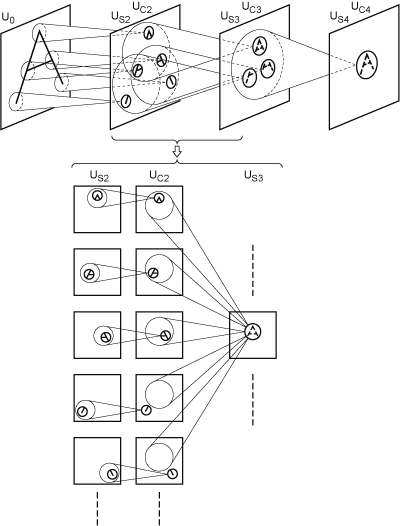
\includegraphics[width=0.72\linewidth]{images/Neocognitron}
		\caption{Der Prozess der Mustererkennung im Neocognitron. Die untere Hälfte der Abbildung ist eine vergrößerte Darstellung eines Teils vom Neocognitron. \protect\cite{neocognitron:scholarpediafig2}}
		\label{fig:neocognitron}
	\end{figure}

	Fukushima führte in seinem Neocognitron-Modell zwei besondere Komponenten ein: \emph{S-Zellen} und \emph{C-Zellen}. Der Einfachheit halber kann man Zellen als Neuronen betrachten. Während S-Zellen zur Merkmalsextraktion dienen, werden C-Zellen in das Neocognitron-Modell eingefügt, um Positionsfehler in den Merkmalen des Stimulus zu berücksichtigen. Die Zellen sind in abwechselnden Schichten von S-Zellen und C-Zellen angeordnet, so dass der Prozess der Merkmalsextraktion durch S-Zellen sowie der Tolerierung der Positionsverschiebung durch C-Zellen in der gesamten Netzwerkarchitektur wiederholt wird. Dadurch lassen sich lokale Merkmale, die in niedrigeren Schichten extrahiert wurden, schrittweise in globalere Merkmale integrieren (siehe \autoref{fig:neocognitron}). Die Schichten von S- sowie C-Zellen im Neocognitron sind jeweils die Vorläufer von den zwei grundlegenden Arten von Schichten in modernen CNN-Architekturen: \emph{Convolutional Layer} und \emph{Pooling Layer} (mehr dazu im \autoref{sec:CNN-Funktionale_Schichten}).
	
	\item[1989 \& 1998]
	
	Obwohl das Neocognitron-Modell 1980 erschien, wurde der Backpropagation-Algorithmus erst fast ein Jahrzehnt später in \cite{yannlecun1989} zum Trainieren von CNN angewendet. Der Autor dieser Veröffentlichung, Yann LeCun, wandte erfolgreich eine Netzwerkarchitektur an, die eine Variante vom Neocognitron-Modell war und durch den Backpropagation-Algorithmus trainiert wurde, um handgeschriebene Postleitzahlen zu identifizieren. Diese Architektur ist die ursprüngliche Form von \emph{LeNet-5}, die als die bekannteste CNN-Architektur angesehen werden kann. LeNet-5 wurde erstmals 1998 in \cite{yannlecun1998} eingeführt. Dabei haben die Autoren verschiedene Methoden zur Erkennung von handschriftlichen Zeichen (einschließlich LeNet-5) überprüft und auf Basis ihrer Leistungen bei einer Standardaufgabe zur Erkennung handschriftlicher Ziffern verglichen. Die Ergebnisse zeigten, dass CNN im Allgemeinen und LeNet-5 im Besonderen alle anderen Modelle übertrafen. Folglich war LeNet-5 in den folgenden Jahren der Ausgangspunkt für viele weitere CNN-Architekturen. Dieses Modell legte den Grundstein für modernes Computer-Vision.
	
	\item[2012]
	
	Jedoch war LeNet-5 aufgrund des Mangels an Rechenressourcen im Jahr 1998 noch nicht in der Lage, auf anspruchsvollere Daten als Ziffern zu skalieren. Um eine hohe Leistung bei komplexen Daten zu erzielen, war es notwendig, dass CNN-Modelle tiefer gehen und mehr Schichten haben, was rechenintensiv war, aber durch den Einsatz von Grafikprozessoren (GPUs) möglich wurde. Diese Schlussfolgerung wurde 2012 von Alex Krizhevsky in \cite{10.1145/3065386} gezogen und durch sein CNN-Modell \emph{AlexNet} demonstriert. AlexNet ist größtenteils LeNet-5 ähnlich, nur viel größer und tiefer (in Bezug auf Größe und Anzahl der Schichten) und wurde mit zwei GPUs trainiert. Daneben war es die erste CNN-Architektur, die Convolutional Layer direkt übereinander stapelte, anstatt wie im Neocognitron-Modell von Fukushima ein Pooling Layer über jedem Convolutional Layer zu stapeln. Mit großem Vorsprung hat diese Architektur den Wettbewerb ILSVRC 2012 gewonnen: Das Modell erreichte 83\% Top-5-Genauigkeit, während das zweitbeste nur 74\% erreichen konnte\footfullcite{imagenet2012result}. Dies war das erste Mal, dass ein CNN-Modell beim großen ImageNet-Datensatz so gut funktionierte. AlexNet gilt somit als eine der einflussreichsten Veröffentlichungen im Bereich Computer-Vision und hat viele weitere Artikel angeregt, die GPUs verwandten, um das Training von CNNs zu beschleunigen.
	
\end{description}

\section{Unterschiede zwischen DNN- und CNN-Struktur}

Wie im vorherigen Kapitel erwähnt ist CNN ein Sondertyp von DNN, der meistens für visuelle Anwendungen verwendet wird. Während die Leistung eines normalen DNN bei der Verarbeitung visueller Eingaben eingeschränkt ist, kann ein CNN dabei aufgrund von \emph{dreidimensionalen Neuronenblocks} und \emph{lokalen Konnektivität} eine hohe Leistung erreichen. 

Jede Schicht in einem normalen DNN lässt sich wie in \autoref{fig:3dcnn} links durch einen eindimensionalen Vektor darstellen. Außerdem ist jedes Neuron mit allen anderen Neuronen sowohl in der vorherigen als auch in der nächsten Schicht verbunden, daher werden DNN-Schichten auch als \emph{Fully-Connected Layers} bekannt. Allerdings ergeben sich zwei Probleme aus der \emph{eindimensionalen Darstellung von Schichten} sowie der \emph{vollen Konnektivität} in DNN. Erstens, wenn die zwei- oder dreidimensionalen Bilder in eindimensionale Vektoren abgeflacht werden, können Zusammenhänge zwischen Pixel, die zusammen ein Objekt im Bild bilden, verloren gehen. Zweitens lassen sich normale DNNs auf großformatige Bilder nicht gut skalieren, da die Anzahl der Gewichte, die zum Trainieren von normalen DNNs mit diesen Bilder benötigt werden, enorm sein kann. Dies kann dazu führen, dass der Computer aufgrund von Out-Of-Memory-Fehler den Trainingsvorgang abbricht.

\begin{figure}[!hb]
	\centering
	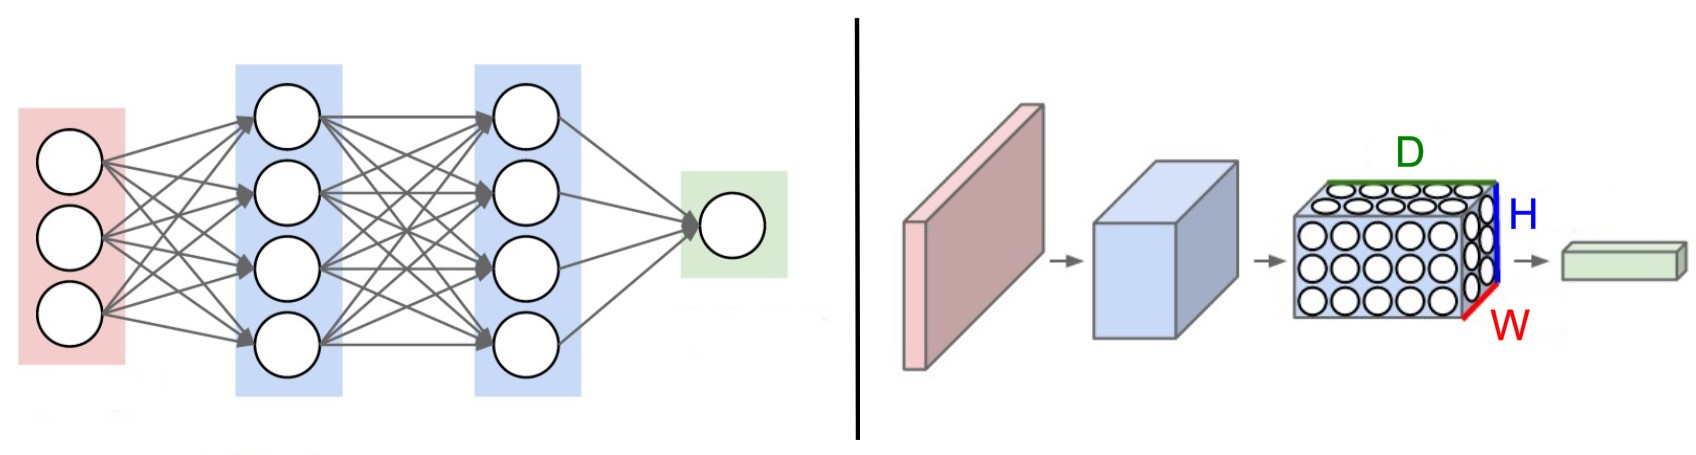
\includegraphics[width=\linewidth]{images/3DCNN}
	\caption{Links: Ein normales DNN. Rechts: Ein CNN ordnet die Neuronen jeder seiner Schichten in drei Dimensionen (Breite - W, Höhe - H, Tiefe - D) an. Beachte, dass sich das Wort ''Tiefe'' hier auf die dritte Dimension eines Neuronenblocks bezieht, nicht auf die Gesamtzahl der Schichten in einem CNN.  \protect\cite{CS231nCNNarchitecture}}
	\label{fig:3dcnn}
\end{figure}

Ein CNN behandelt diese beiden Probleme, indem es dreidimensionale sowie teilweise verbundene Schichten in seiner Struktur verwendet:

\begin{description}
	\item[3D-Neuronenblocks]
	
	Wie der Name schon andeutet, wird jede Schicht eines CNN wie in \autoref{fig:3dcnn} rechts als dreidimensionaler Neuronenblock dargestellt. Die drei Dimensionen der Eingabeschicht entsprechen jeweils der Höhe, Breite sowie Anzahl der Farbkanäle vom Eingabebild. Diese Darstellung sorgt dafür, dass die Zusammenhänge zwischen Pixel im Eingabebild unverändert bleiben, was in normalem DNN nicht möglich ist.

	\item[Lokale Konnektivität]
	
	CNN ist so aufgebaut, dass jedes Neuron in einer Schicht nur mit einem kleinen Bereich der vorherigen Schicht (rezeptiven Feld) verbunden ist, anstatt vollständig mit allen Neuronen davon verbunden zu sein. Diese Organisation stammt aus der Hierarchical-Neural-Network-Idee von Hubel und Wiesel. Dadurch lässt sich die Anzahl der zu trainierenden Gewichte deutlich verringern, was die Skalierung von CNNs auf Großbilder ermöglicht.
	
\end{description}

\section{Funktionale Schichten} \label{sec:CNN-Funktionale_Schichten}

Aus funktionaler Sicht bezieht sich eine CNN-Schicht auf eine bestimmte Transformation und deren Ergebnis (siehe \autoref{fig:CNN_funktionale_schicht}). Im Allgemeinen sind sowohl die Eingaben als auch die Ausgaben jeder Transformation dreidimensionale Neuronenblocks, die als Stapeln von \emph{Feature-Maps} betrachtet werden können. Bei einem Feature-Map handelt es sich um eine zweidimensionale Karte, die Merkmale kodiert, die durch Transformieren bestimmter Merkmale des Eingabeblocks erhalten werden. Je nach Art der Transformation unterscheidet man zwischen zwei Grundtypen von CNN-Schichten, nämlich Convolutional Layer und Pooling Layer.

\begin{figure}[!hb]
	\centering
	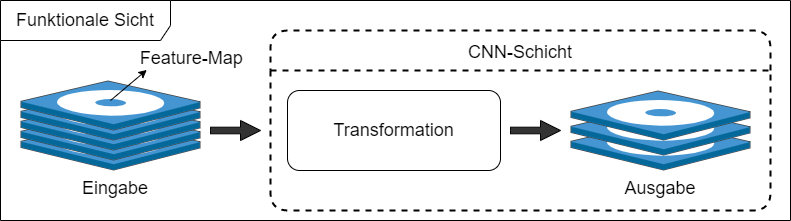
\includegraphics[width=\linewidth]{images/CNN_funktionale_schicht}
	\caption{CNN-Schicht aus funktionaler Sicht}
	\label{fig:CNN_funktionale_schicht}
\end{figure}

\subsection{Convolutional Layer}

Wie die S-Zellen-Schichten im Neocognitron-Modell von Fukushima werden Convolutional Layers für die Merkmalsextraktion verwendet. Ein Convolutional Layer transformiert dazu Feature-Maps bzw. Merkmale im Eingabeblock in neue Feature-Maps mit komplexeren nützlicheren Merkmalen (siehe \autoref{fig:ConvLayerTransformation}).
	
\begin{figure}[!hb]
	\centering
	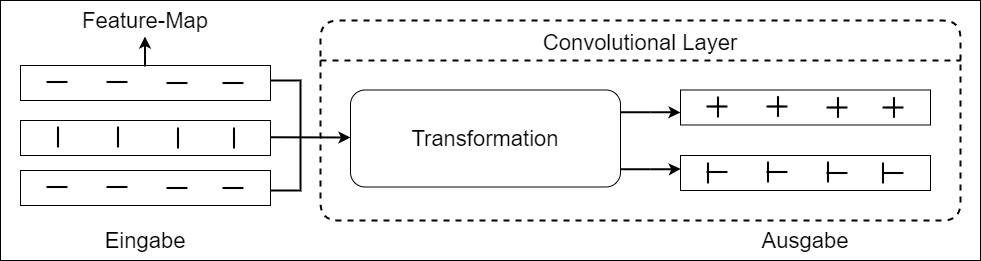
\includegraphics[width=\linewidth]{images/ConvLayerTransformation}
	\caption{Transformation in Convolutional Layer}
	\label{fig:ConvLayerTransformation}
\end{figure}
	
Die Transformation in Convolutional Layer lässt sich durch sogenannte \emph{Filter} durchführen. Wie der Name bereits verrät, werden während der Transformation mehrere Filter auf den ganzen Eingabeblock angewendet, und alle visuellen Merkmale darin, die den in diesen Filter angegebenen Merkmalen am ähnlichsten sind, werden extrahiert und in neue Feature-Maps integriert (siehe \autoref{fig:ConvLayerTransformationFilter}). In der Regel gilt, dass sich aus jedem Filter ein Feature-Map im Ausgabeblock ergibt.
	
\begin{figure}[h]
	\centering
	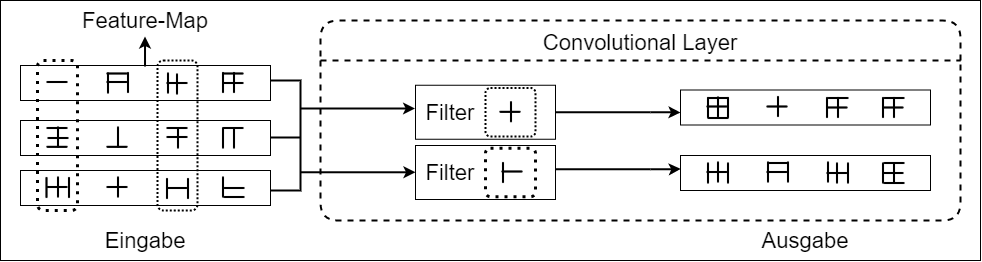
\includegraphics[width=\linewidth]{images/ConvLayerTransformationFilter}
	\caption{Filter in Convolutional Layer}
	\label{fig:ConvLayerTransformationFilter}
\end{figure}

Das Merkmal, das in einem Filter angegeben ist, wird ihm nicht manuell zugewiesen, sondern muss automatisch während des Trainingsvorgangs vom CNN gelernt werden. In der Tat ist ein Filter eine Zusammenstellung von Verbindungsgewichte, die mit dem Backpropagation-Algorithmus zu optimieren sind. Während des Trainings findet ein CNN die nützlichsten Filter für seine Aufgabe und lernt, diese zu komplexeren Merkmalen zu kombinieren.

Die \autoref{fig:convlayer} bildet die Merkmalsextraktion in Convolutional Layer in beiden funktionalen und strukturellen Hinsichten ab. Mehr Informationen dazu befinden sich in \cite{10.5555/3378999}.

\begin{figure}[h]
		\centering
		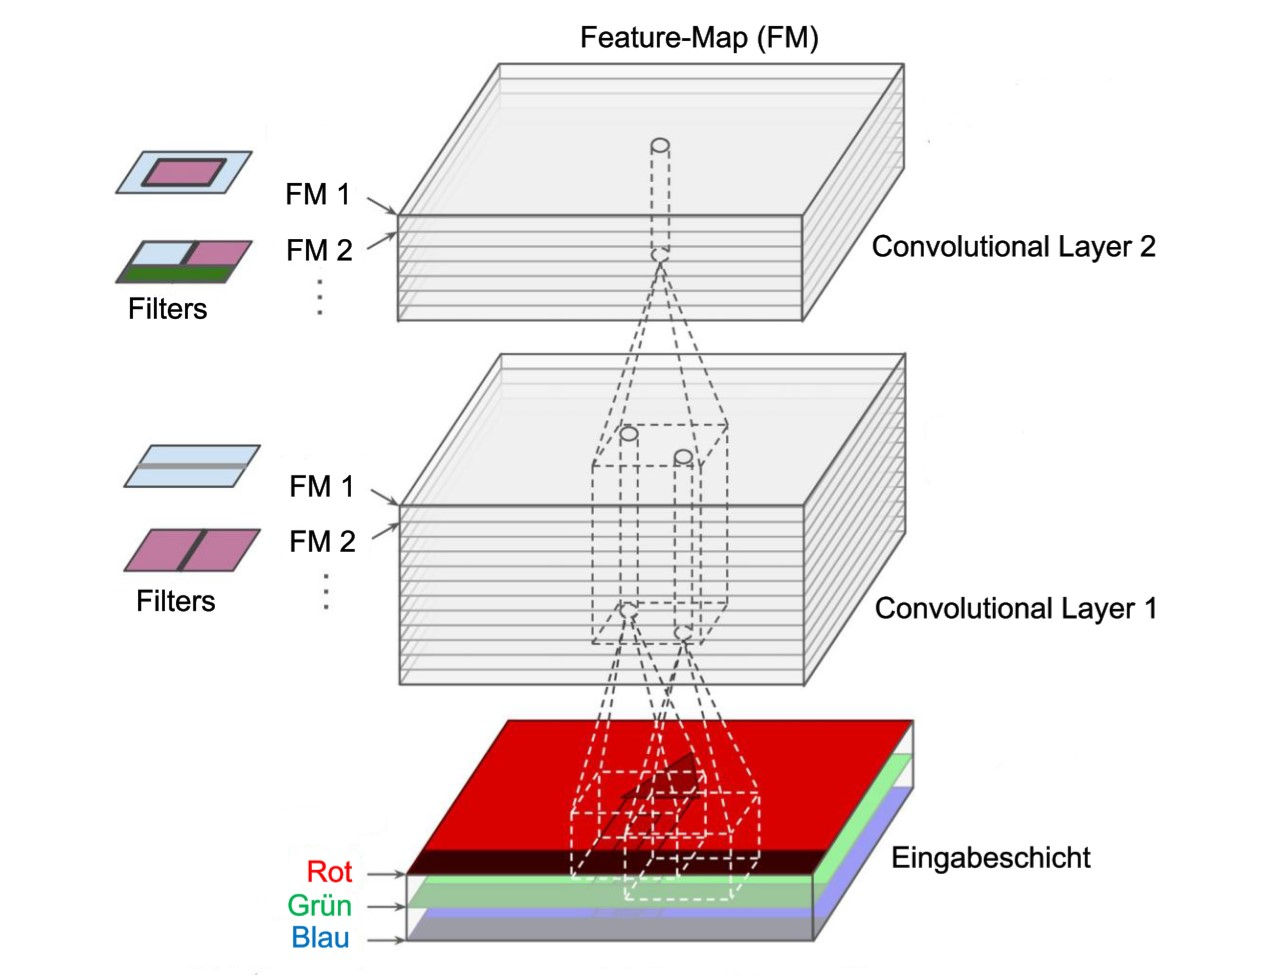
\includegraphics[width=\linewidth]{images/convolutionalLayer}
		\caption{Merkmalsextraktion in Convolutional Layer  \protect\cite{convlayer}}
		\label{fig:convlayer}
\end{figure}
	

\subsection{Pooling Layer}
	
Pooling Layers dienen nicht nur zur Tolerierung der Positionsverschiebung wie die C-Zellen-Schichten im Neocognitron-Modell, sondern auch zur Reduzierung der Rechenlast, Speichernutzung und Anzahl der Verbindungsgewichte. Diese Ziele lassen sich durch Unterabtasten (d.h. Schrumpfen) des Eingabeblocks erreichen. In anderen Worten, ein Pooling Layer transformiert Feature-Maps im Eingabeblock in kleinere Feature-Maps aber mit den gleichen Merkmalen (siehe \autoref{fig:PoolingLayerTransformation}).
	
\begin{figure}[!hb]
	\centering
	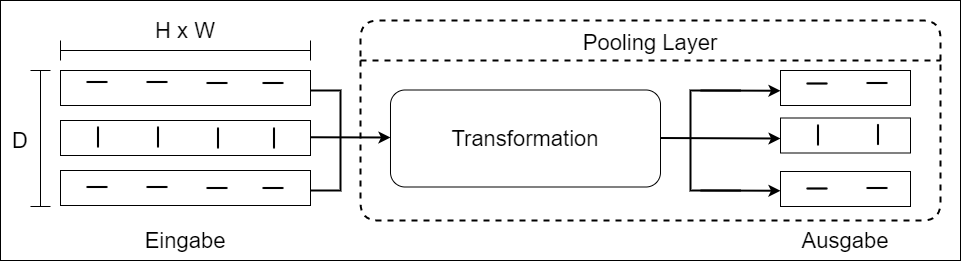
\includegraphics[width=\linewidth]{images/PoolingLayerTransformation}
	\caption{Transformation in Pooling Layer}
	\label{fig:PoolingLayerTransformation}
\end{figure}

Die Transformation in Pooling Layer lässt sich auch durch Filter durchführen. Es gilt ebenfalls die Regel, dass sich aus jedem Filter ein Feature-Map im Ausgabeblock ergibt. Trotzdem haben diese Filter im Gegensatz zu denjenigen in Convolutional Layer keine Verbindungsgewichte, d.h. sie lernen während des Trainings gar nicht, sondern wenden lediglich eine der Aggregatfunktionen auf die Feature-Maps an, um Merkmale darin zu aggregieren und dadurch die Größe der Feature-Maps zu verkleinern. Beispielsweise in \autoref{fig:PoolingLayerTransformationFilter} wird ein Filter der Art $MAX()$ oder $AVG()$ zunächst auf die ersten drei Merkmale jedes Feature-Map angewendet und anschließend auf die letzten drei (Jeder Strich entspricht einem Merkmal). Die resultierenden Feature-Maps haben dank der Aggregation zwei gleiche Merkmale und sind somit nur halb so groß wie zuvor.

\begin{figure}[!hb]
	\centering
	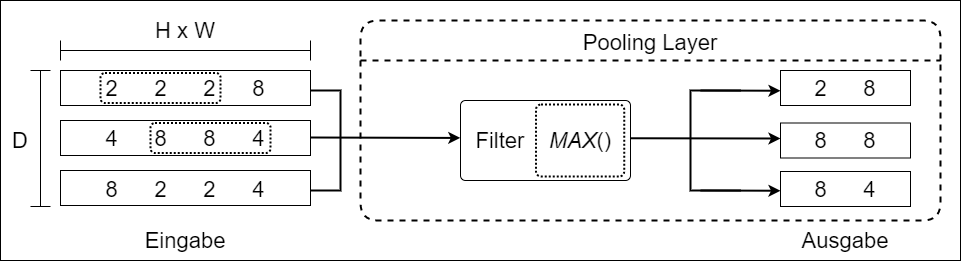
\includegraphics[width=\linewidth]{images/PoolingLayerTransformationFilter}
	\caption{Filter in Pooling Layer}
	\label{fig:PoolingLayerTransformationFilter}
\end{figure}

Typischerweise werden Convolutional und Pooling Layers zusammen mit Fully-Connected Layers kombiniert und in einer bestimmten Reihenfolge angeordnet, um ein CNN-Modell z.B. zur Bildklassifizierung aufzubauen (siehe \autoref{fig:imgKlassifizierungProzess}). Wenn das Eingabebild die Schichten in einem solchen CNN-Modell durchläuft, wird das Bild immer kleiner, aber aufgrund von Convolutional Layers immer tiefer (d.h. es gibt mehr Feature-Maps). In diesem Modell hält die Eingabeschicht die rohen Pixelwerte vom Eingabebild, während die Ausgabeschicht mittels \emph{Softmax-Funktion}\footfullcite{Softmax} einen eindimensionalen Vektor der Größe $K$ (Anzahl der Klassen) ausgibt, wobei jeder Komponentenwert einer Wahrscheinlichkeit entspricht, dass das Eingabebild zu einer bestimmten Klasse gehört. 

\begin{figure}[!hb]
	\centering
	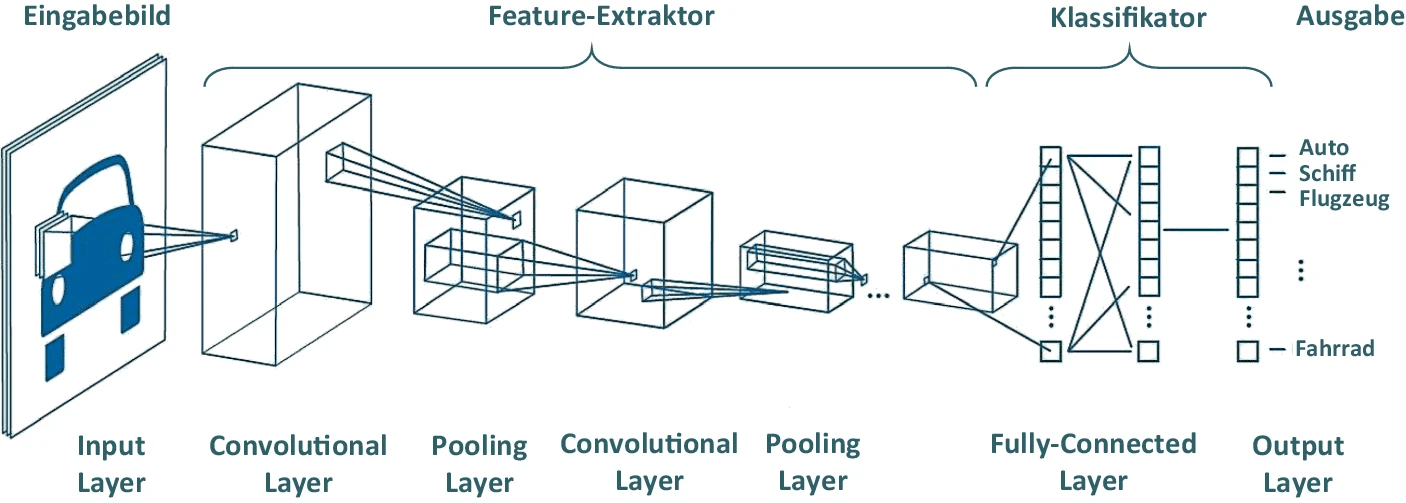
\includegraphics[width=\linewidth]{images/imgKlassifizierungProzess}
	\caption{Allgemeiner Aufbau eines CNN \protect\cite{Zschech2021}}
	\label{fig:imgKlassifizierungProzess}
\end{figure}
% \section{Photofallen}
%technische specs der Kameras.

%Was sind Kamerafallen

%Wo gesetzt

%Automatische Arbeit von Umweltmodellierung
